\newcommand{\deltaT}[0]{$\delta{}t$}
\newcommand{\deltaX}[0]{$\delta{}x$}
\newcommand{\deltaY}[0]{$\delta{}y$}

\section{An Example Simulation Tick}\label{sec:Research:SimulationTick}
The 1998 book ``Numerical simulation in fluid dynamics : a practical introduction''\cite{book:griebel1998numerical} defines a basic structure for a discrete simulated timestep (a.k.a. a ``tick'') and provides a sample guide to implementing it in Fortran or C.
To the best of the author's knowledge this was used as the base of the ACA coursework, and continues to be the base of this project.
This section will explain the general structure of the simulation as defined in \cite{book:griebel1998numerical}.

The simulation described specifically simulates ``\emph{laminar} flows of \emph{viscous, incompressible fluids}''\cite{book:griebel1998numerical} in 2D.
\emph{Laminar} flows can be treated as separate layers of particles that can slide past each other, which interact solely through friction forces.
The opposite of this is Turbulent flow, where particles may move between layers due to small friction forces\cite{book:griebel1998numerical}.
This adds extra viscosity (the turbulent eddy viscosity, as covered in more detail in \cite{bird2006transport}) which is much more difficult to accurately model.

\emph{Incompressible} fluids have a uniform density across the entire flow, which greatly simplifies the calculations.
This property can be assumed for low-velocity gases, and for most liquids\cite{book:griebel1998numerical}.

\emph{Viscous} fluids have high internal friction forces that will eventually bring a moving fluid to rest.
The viscosity is controlled by a parameter known as the Reynolds number $Re$\cite{falkovich2018fluid}, which is constant over the fluid.
As $Re \to 0$ the viscosity of the fluid approaches infinity, and as $Re \to \infty$ the fluid becomes \emph{inviscid}, i.e. not viscous.
Using high $Re$ this sim could be used to simulate inviscid fluids, although it is important for the fluid to still be laminar and incompressible.

Any forces acting throughout the bulk of the fluid i.e. gravity can be simulated using the $g = (g_x, g_y)$ vector.
However the 2D variant of the simulation has been used in this project for top-down simulations with a level plane, so this is left unused.

\subsection{The Simulation Variables}
The simulation solves for three variables: horizontal velocity $u$, vertical velocity $v$, and pressure $p$.
These variables are related by the Navier-Stokes momentum and continuity equations, which can be written as follows:
\newcommand{\partialderiv}[2]{\frac{\partial{#1}}{\partial{#2}}}
\newcommand{\paren}[1]{\left(#1\right)}
\begin{equation}
\begin{aligned}
    \partialderiv{u}{t} + \partialderiv{p}{x} &= \frac{1}{Re}\paren{ \partialderiv{^2u}{x^2} + \partialderiv{^2u}{y^2}} - \partialderiv{(u^2)}{x} - \partialderiv{(uv)}{y} + g_x, \\
    \partialderiv{v}{t} + \partialderiv{p}{y} &= \frac{1}{Re}\paren{ \partialderiv{^2v}{x^2} + \partialderiv{^2v}{y^2}} - \partialderiv{(uv)}{x} - \partialderiv{(v^2)}{y} + g_y
    \label{eq:NavierStokesMomentum}
\end{aligned}
\end{equation}
\begin{equation}
\label{eq:NavierStokesContinuity}
    \frac{\partial{u}}{\partial{x}} + \frac{\partial{v}}{\partial{y}} = 0
\end{equation}
The values of the simulated quantities at tick $\#n$ are represented by $u^{(n)}, v^{(n)}, p^{(n)}$.
These values are discretized by evaluating them at points on a staggered grid (see \cref{fig:staggered_grid}).
This grid is indexed by $i$ in the x-direction and $j$ in the y-direction.
It is important to note the variables $u,v$ represent the current velocity of the fluid within each grid space, \textbf{not} the velocity of the grid cells themselves.
The grid does not move at any point during the simulation.

\begin{figure}[ht]
\centering
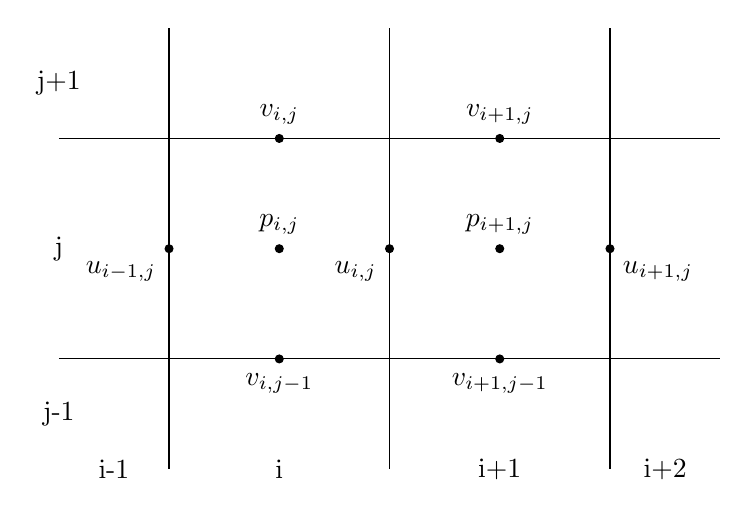
\begin{tikzpicture}[scale=1.4]

\draw (0, 1) -- (6, 1);
\draw (0, 3) -- (6, 3);

\draw (1,4) -- (1,0);
\draw (3,4) -- (3,0);
\draw (5,4) -- (5,0);

\node at (0, 0.5) {j-1}; 
\node at (0, 2) {j}; 
\node at (0, 3.5) {j+1};

\node at (0.5, 0) {i-1}; 
\node at (2, 0) {i}; 
\node at (4, 0) {i+1};
\node at (5.5, 0) {i+2};

\node[label=above:{$p_{i,j}$}, draw, circle, fill, minimum size=0.1cm, inner sep=0pt] at (2, 2) {};
\node[label=above:{$p_{i+1,j}$}, draw, circle, fill, minimum size=0.1cm, inner sep=0pt] at (4, 2) {};

\node[label=below left:{$u_{i-1,j}$}, draw, circle, fill, minimum size=0.1cm, inner sep=0pt] at (1, 2) {};
\node[label=below left:{$u_{i,j}$}, draw, circle, fill, minimum size=0.1cm, inner sep=0pt] at (3, 2) {};
\node[label=below right:{$u_{i+1,j}$}, draw, circle, fill, minimum size=0.1cm, inner sep=0pt] at (5, 2) {};

\node[label=above:{$v_{i,j}$}, draw, circle, fill, minimum size=0.1cm, inner sep=0pt] at (2, 3) {};
\node[label=above:{$v_{i+1,j}$}, draw, circle, fill, minimum size=0.1cm, inner sep=0pt] at (4, 3) {};

\node[label=below:{$v_{i,j-1}$}, draw, circle, fill, minimum size=0.1cm, inner sep=0pt] at (2, 1) {};
\node[label=below:{$v_{i+1,j-1}$}, draw, circle, fill, minimum size=0.1cm, inner sep=0pt] at (4, 1) {};

\end{tikzpicture}
    \caption{Discretization points for each variable on the staggered grid\cite{book:griebel1998numerical}}
    \label{fig:staggered_grid}
\end{figure}

Each of the variables is located at a different position on the grid cell.
Horizontal velocity $u_{i,j}$ is at the midpoint of the right cell edge, vertical velocity $v_{i,j}$ is at the midpoint of the top cell edge, and pressure $p_{i,j}$ is at the midpoint of the cell.
% Staggering the variables in this manner avoids oscillation in the pressure value caused by odd-even decoupling.
This is used to solve odd-even decoupling\cite{Harlow1965NumericalSurface}: for a fluid at rest (i.e. $u = v = 0$) the continuous solution is that the pressure $p$ is a constant across the grid.
However were this to be discretized using central differences with all variables in the same locations, it would also be possible for a checkerboard of pressure values to form, and for oscillation to take place\cite{book:griebel1998numerical}.
This is prevented by staggering the variables.
\cite{peric1988comparison} shows that this is also preventable through colocated grids, where a single grid is used for all variables and the velocities of each side of the cell are found using interpolation.
These cell sides are implicitly staggered relative to the pressure and so avoid this problem.

To allow for derivatives to be accurately calculated for cells on the edges of the grid, boundary cells are added around each grid.%\todomark{figure}
The cells on the edges of any obstacles in the simulation are also marked as boundary squares.
For a finite domain of size $(imax, jmax)$ this leads to a final grid size of $(imax + 2)$ by $(jmax + 2)$, where valid fluid values fall in the ranges %
%$1 \leq i \leq imax$, $1 \leq j \leq jmax$
$i \in \{1..imax\}$, $j \in \{1..jmax\}$.

The physical dimensions of each grid space are represented by \deltaX{}, \deltaY{}.
This allows the derivatives of $u$ and $v$ to be calculated by finding the centered differences.
\begin{align}
    \left[\frac{\partial{u}}{\partial{x}}\right]_{i,j} := \frac{u_{i,j}-u_{i-1,j}}{\delta{x}}, 
    & \quad %
    \left[\frac{\partial{v}}{\partial{y}}\right]_{i,j} := \frac{v_{i,j}-v_{i,j-1}}{\delta{y}}
\end{align}
% TODO multicolumn
% \begin{multicols}{2}
%   \begin{equation}
%     a=b
%   \end{equation}\break
%   \begin{equation}
%     b=c
%   \end{equation}
% \end{multicols}
The partial derivatives for pressure $\partial{p}/\partial{x}, \partial{p}/\partial{y}$ are found in the same way.
The remaining derivatives, including second derivatives and $\partial{uv}/\partial{x}, \partial{uv}/\partial{y}$, can also be discretized by taking the difference across midpoints of their respective dimensions\cite{hirt1976}.
%

\subsection{Simulation Stages}
\begin{figure}[ht]
    \centering

    \begin{tikzpicture}[
    scale=0.8, every node/.style={scale=0.8},
    stage/.style={minimum height = 2.5em, draw, anchor=north}
    ]
        \newcommand{\stagesep}{-0.4};
        \node[stage](s1) at (0,0) {Compute $\delta{t}$};
        \node[stage](s2) at ($(s1.south) + (0,\stagesep)$) {Compute Tentative Velocity};
        \node[stage](s3) at ($(s2.south) + (0,\stagesep)$) {Compute Poisson RHS};
        \node[stage](s4) at ($(s3.south) + (0,\stagesep)$) {Poisson Solver};
        % \node[stage](s5) at ($(s4.south) + (0,-0.6)$) {Poisson Iteration \#2};
        % \node[stage](s6) at ($(s5.south) + (0,-0.6)$) {...};
        % \node[stage](s7) at ($(s6.south) + (0,-0.6)$) {Poisson Iteration \#N};
        \node[stage](s8) at ($(s4.south) + (0,\stagesep)$) {Update Velocity};
        \node[stage](s9) at ($(s8.south) + (0,\stagesep)$) {Boundary Conditions};
    
        \draw[thick, ->] (s4.east) arc (0:-330:-0.4cm);% syntax (starting point coordinates) arc (starting angle:ending angle:radius)
        \node at ($(s4.east) + (2cm, 0)$){$N$ {}iterations}; 
    
        \draw[-latex] (s1.south) -- (s2.north);
        \draw[-latex] (s2.south) -- (s3.north);
        \draw[-latex] (s3.south) -- (s4.north);
        \draw[-latex] (s4.south) -- (s8.north);
        % \draw[-latex] (s5.south) -- (s6.north);
        % \draw[-latex] (s6.south) -- (s7.north);
        % \draw[-latex] (s7.south) -- (s8.north);
        \draw[-latex] (s8.south) -- (s9.north);
    \end{tikzpicture}
    \caption{Stages of a Simulation Tick}
    \label{fig:SimStages}
\end{figure}
Each simulation tick can be split into multiple stages, shown in \cref{fig:SimStages}.
These stages are described in detail in the following sections.

\subsection{Timestep Calculation}
\label{sec:TimestepCalculation}
Each simulation tick simulates a discrete amount of time known as a timestep \deltaT{}.
This timestep is not a fixed value, and typically one would want to select as large a timestep as possible.
However, there are constraints on it's maximum value which depend on the simulation state.

As the derivatives are calculated between adjacent grid points, it is impossible to accurately simulate a timestep where fluid moves between non-adjacent grid cells \todoref{Figure?}.
%[Peyret&Taylor,1983]or[Roache,1976].Anadaptivestepsizecontrolbasedonthesestabilityconditionsis usedin[Tome&McKee,1994].
% The simulation cannot accurately solve a timestep in which particles move completely over a cell (see Figure \todocite{}).
To prevent this the timestep \deltaT{} is calculated from the fluid velocities to make it impossible.
\begin{equation}
    \delta{t} = \tau * \text{min}\left(
        \frac{Re}{2}\left(
            \frac{1}{\delta{x}^2} + \frac{1}{\delta{y}^2}
        \right)^{-1},
        \frac{\delta{x}}{|u_{max}|},
        \frac{\delta{y}}{|v_{max}|}
    \right)
\end{equation}

Because the new velocities calculated in this tick may be larger than $u_{max}$ and $v_{max}$, the safety factor $\tau \in [0, 1]$ is used to ensure the timestep is large enough to account for it\cite{TOME1994171}.

\subsection{Tentative Velocity}
The final values of $u$ and $v$ are defined as
\begin{equation}
\begin{aligned}
    u^{(n+1)} &= u^{(n)} + \delta{t}
    \left[
        \frac{1}{Re}
        \paren{\partialderiv{^2u}{x^2} + \partialderiv{^2u}{y^2}} - \partialderiv{(u^2)}{x} - \partialderiv{(uv)}{y} + g_x - \partialderiv{p}{x}
    \right] \\
    v^{(n+1)} &= v^{(n)} + \delta{t}
    \left[
        \frac{1}{Re}
        \paren{\partialderiv{^2v}{x^2} + \partialderiv{^2v}{y^2}} - \partialderiv{(uv)}{x} - \partialderiv{(v^2)}{y} + g_y - \partialderiv{p}{y}
    \right]
\end{aligned}
\end{equation}
However, as these depend on the partial derivatives of $p$, which itself depends on velocity, they cannot be solved analytically.
In order to iteratively find $p$ the variables $f$ and $g$, for horizontal and vertical ``tentative velocity'', are introduced.
\begin{equation}
\begin{aligned}
    f^{(n)} := u^{(n)} + \delta{t}
    \left[
        \frac{1}{Re}
        \paren{\partialderiv{^2u}{x^2} + \partialderiv{^2u}{y^2}} - \partialderiv{(u^2)}{x} - \partialderiv{(uv)}{y} + g_x
    \right] \\
    g^{(n)} := v^{(n)} + \delta{t}
    \left[
        \frac{1}{Re}
        \paren{\partialderiv{^2v}{x^2} + \partialderiv{^2v}{y^2}} - \partialderiv{(uv)}{x} - \partialderiv{(v^2)}{y} + g_y
    \right]
\end{aligned}
\end{equation}
\begin{equation}
\begin{aligned}
    u^{(n+1)} = f^{(n)} - \delta{t}\frac{\partial{p^{(n+1)}}}{\partial{x}} \\
    v^{(n+1)} = g^{(n)} - \delta{t}\frac{\partial{p^{(n+1)}}}{\partial{y}}
    \label{eq:uv_modified}
\end{aligned}
\end{equation}

\subsection{Solving the Poisson Equation with SOR}
\label{sec:SimulationPoisson}
% Two phases - calculating the RHS, then solving
For continuity to be achieved, the final velocity values must fulfil the continuity equation (\cref{eq:NavierStokesContinuity}), the time discretization of which is shown below:
\begin{equation}
    \frac{\partial{u^{(n+1)}}}{\partial{x}} + \frac{\partial{v^{(n+1)}}}{\partial{y}} = 0
\end{equation}
This means that the total amount of fluid entering a cell in tick $n+1$ is equal to the amount of fluid leaving, which must be the case otherwise the amount of fluid per cell wouldn't be constant and the fluid would be compressed.

Substituting the formulae in \cref{eq:uv_modified} into this relation and rearranging gives
\begin{equation}
    \frac{\partial^2{p^{(n+1)}}}{\partial{x^2}} + \frac{\partial^2{p^{(n+1)}}}{\partial{y^2}} = \frac{1}{\delta{t}}\left(\frac{\partial{f^{(n)}_{i,j}}}{\partial{x}} + \frac{\partial{g^{(n)}_{i,j}}}{\partial{y}}\right)
\end{equation}
The right hand side of this equation is constant for timestep $n$, so can be precalculated and assigned to its own variable $rhs$.
\begin{equation}
rhs_{i,j} := \frac{1}{\delta{t}}\left(\frac{\partial{f^{(n)}_{i,j}}}{\partial{x}} + \frac{\partial{g^{(n)}_{i,j}}}{\partial{y}}\right)
\end{equation}
\begin{equation}
\frac{\partial^2{p^{(n+1)}}}{\partial{x^2}} + \frac{\partial^2{p^{(n+1)}}}{\partial{y^2}} = rhs_{i,j}
\end{equation}
Discretizing this gives
\newcommand{\discretized}[4]{#1^{#2}_{#3,#4}}
\newcommand{\pdisc}[3]{\discretized{p}{(#1)}{#2}{#3}}
\newcommand{\fdisc}[3]{\discretized{f}{(#1)}{#2}{#3}}
\newcommand{\gdisc}[3]{\discretized{g}{(#1)}{#2}{#3}}
\newcommand{\ebounds}[1]{\discretized{\epsilon}{#1}{i}{j}}
\begin{multline}
    \frac{\pdisc{n+1}{i+1}{j} - 2\pdisc{n+1}{i}{j} + \pdisc{n+1}{i-1}{j}}
    {(\delta{x})^2} + 
    \frac{\pdisc{n+1}{i}{j+1} - 2\pdisc{n+1}{i}{j} + \pdisc{n+1}{i}{j-1}}
    {(\delta{y})^2}
    % = \frac{1}{\delta{t}}\paren{
    %     \frac{\fdisc{n}{i}{j} - \fdisc{n}{i-1}{j}}{\delta{x}} + 
    %     \frac{\gdisc{n}{i}{j} - \gdisc{n}{i}{j-1}}{\delta{y}}
    % }
    = rhs_{i,j}
\end{multline}
and taking the simplest boundary conditions\cite{book:griebel1998numerical}
\begin{align}
    p_{0,j} &= p_{1,j}, & p_{i_{max+1},j} &= p_{i_{max},j} & j \in \{1..j_{max}\} \\
    p_{i,0} &= p_{i,1}, & p_{i,j_{max+1}} &= p_{i,j_{max}} & i \in \{1..i_{max}\} \\
    f_{0,j} &= u_{0,j}, & f_{i_{max},j} &= u_{i_{max},j} & j \in \{1..j_{max}\} \\
    g_{i,0} &= v_{i,0}, & g_{i,j_{max}} &= v_{i,j_{max}} & i \in \{1..i_{max}\}
\end{align}
resolves the equation to:
\begin{multline}
    \frac{\ebounds{E}(\pdisc{n+1}{i+1}{j} - \pdisc{n+1}{i}{j}) - \ebounds{W}(\pdisc{n+1}{i}{j} - \pdisc{n+1}{i-1}{j})}
    {(\delta{x})^2} \\
    + \frac{\ebounds{N}(\pdisc{n+1}{i}{j+1} - \pdisc{n+1}{i}{j}) - \ebounds{S}(\pdisc{n+1}{i}{j} - \pdisc{n+1}{i}{j-1})}
    {(\delta{y})^2}\\
    % = \frac{1}{\delta{t}}\paren{
    %     \frac{\fdisc{n}{i}{j} - \fdisc{n}{i-1}{j}}{\delta{x}} + 
    %     \frac{\gdisc{n}{i}{j} - \gdisc{n}{i}{j-1}}{\delta{y}}
    % }
    = rhs_{i,j}
    \label{eq:poisson_pre_sor}
\end{multline}
where $\epsilon_{i,j}^{\{N,S,E,W\}}$ represents the boundary squares (shown here for North, but it extends to the other directions)
\begin{equation}
    \epsilon_{i,j}^{N} = \begin{cases}
        0 & \text{The square directly above $i,j$ is a boundary}\\
        1 & \text{The square directly above $i,j$ is \emph{not} a boundary}
   \end{cases}
\end{equation}


\begin{figure}[t]
\centering
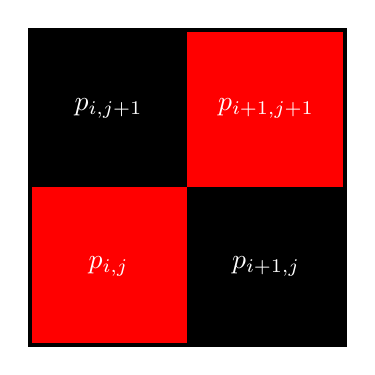
\begin{tikzpicture}[scale=1]
\draw[ultra thick, fill=red] (0,0) rectangle (4,-4);
    \foreach \row in {0,1} {
        \foreach \column in {0} {
    \fill ({4*\column + mod(\row,2)*2}, -\row*2) rectangle +(2,-2);
        }
    }
% \matrix (m) at (0,0) [matrix of nodes,nodes={},
%   anchor=north west,column sep={2cm,between origins},
%   row sep={2cm,between origins}] {
%  {\color{white}{$p_{i,j+1}$}} & {$p_{i+1,j+1}$} \\
%  {$p_{i,j}$} & {\color{white}{$p_{i+1,j}$}} \\
% };
\node at (1,-1) {\color{white}{$\bm{p_{i,j+1}}$}};
\node at (1,-3) {\color{white}{$\bm{p_{i,j}}$}};
\node at (3,-1) {\color{white}{$\bm{p_{i+1,j+1}}$}};
\node at (3,-3) {\color{white}{$\bm{p_{i+1,j}}$}};

% \matrix[matrix of nodes,nodes={draw}]{A & B & C & D & E\\f & G & H & I & J};
\end{tikzpicture}
    \caption{Example checkerboard pattern used for red/black splitting}
    \label{fig:redblack_checkerboard}
\end{figure}
Over the whole grid, this results in a linear system of equations over the inputs $p_{i,j} \forall i \in \{1..i_{max}\}, j \in \{1..j_{max}\}$.
These can be decoupled by partitioning $p$ into red and black squares by a checkerboard pattern (see \cref{fig:redblack_checkerboard}).
As each individual cell only depends on the adjacent values, iterations of Successive Over-Relaxation (SOR) can be performed on red and black in turn to reach a final value\footnote{This could equally be done without partitioning $p$, but the partitioning splits the SOR into separate phases which can then be parallelized. Normal SOR cannot be parallelized\cite{Adams1982AMS}.}\cite{young1971iterative}:
\begin{equation}
    \beta_{i,j} := \frac{\omega}{\left(\frac{\epsilon_{i,j}^E+\epsilon_{i,j}^W}{(\delta{x})^2} + \frac{\epsilon_{i,j}^N+\epsilon_{i,j}^S}{(\delta{y})^2}\right)}
    \label{eq:poisson_beta}
\end{equation}
\begin{multline}
    p^{it+1}_{i,j} := (1 - \omega)p^{it}_{i,j} + \\
    \beta_{i,j} * \left(
    \frac{\epsilon_{i,j}^E p^{it}_{i+1,j}+\epsilon_{i,j}^W p^{it}_{i-1,j}}{(\delta{x})^2} + 
    \frac{\epsilon_{i,j}^N p^{it}_{i,j+1}+\epsilon_{i,j}^W p^{it}_{i,j-1}}{(\delta{y})^2} -
    rhs_{i,j}
    \right)
    \label{eq:poisson_final}
\end{multline}

These iterations are continued until the L2 norm\cite{l2norm} of the residuals (the difference between the left-hand side as calculated and the expected right-hand side of \cref{eq:poisson_final} for each cell) falls below a specific tolerance\footnote{In the ACA coursework this tolerance was relative to the L2 norm of $p$, although this was not directly specified by the book.}\cite{book:griebel1998numerical}.

\subsection{Final Velocity Calculations}
% Update Velocity, applyBoundaryConditions
Once the final values of $p$ have been calculated the velocity values $u,v$ can be found with \cref{eq:uv_modified}.
The boundary conditions for velocity must then be applied.
There are four relevant types of boundary condition\footnote{The book specifies five, including a Periodic Boundary Condition, which the ACA system does not support.}, which are applied depending on the type of boundary.
\begin{enumerate}
    \item No-Slip condition - no fluid penetrates the boundary, and fluid does not move past it i.e. the boundary applies friction.
    \item Free-Slip condition - fluid may not penetrate the boundary, but no friction is applied. Only tangential velocity is preserved for adjacent fluids.
    \item Inflow - fluid is flowing in constantly, so the velocity is set to a constant value. 
    \item Outflow - velocity perpendicular to the surface is preserved and fluids may flow out.
\end{enumerate}
% \todopending{Might need equations here?}

% \subsection{Overall Simulation Pipeline}
